% ============================================================
% Capítulo II (Volumen II) — Teoría electromagnética de la luz.
% Comparación con la teoría elástica
% Traducción de "Théorie mathématique de la lumière II" (1892)
% Original: §§12-20, páginas impresas 19-33
% ============================================================
\chapter{Teoría electromagnética de la luz. Comparación de esta teoría con
la teoría elástica}
\chaptermark{Teoría electromagnética de la luz}
\label{cap:vol2-electromagnetica}

\section{Notación y ecuaciones de Maxwell}

\noindent\textbf{12.} Emplearé en todo lo que sigue las notaciones de
Maxwell, que recuerdo sucintamente, remitiendo para más detalles a la
propia obra del sabio inglés y a mi tratado titulado \emph{Électricité et
Optique}.

Consideremos primero la \emph{fuerza magnética}, cuyas componentes designa
Maxwell por $\alpha,\beta,\gamma$. En seguida, la \emph{inducción
magnética}, cuyas componentes son $a,b,c$ (cf. \emph{Électricité et
Optique}, t.~I, pp.~110 y sig.).

Se tiene, si no hay fuerza coercitiva:
\[
a=\mu\alpha,\qquad b=\mu\beta,\qquad c=\mu\gamma,
\]
siendo $\mu$ el coeficiente de permeabilidad magnética del medio.

En el vacío $\mu=1$. En los cuerpos diamagnéticos, se tiene $\mu<1$, y en
los cuerpos magnéticos $\mu>1$. Pero en la mayoría de los cuerpos, salvo el
hierro, el níquel y el cobalto, $\mu$ es extremadamente próximo a $1$.

Las experiencias de Hertz parecen demostrar además que, en el caso de las
corrientes oscilantes con extrema rapidez, la inducción no tiene tiempo de
producirse y todo ocurre como si $\mu$ fuera igual a $1$. La teoría
electromagnética supone precisamente que los fenómenos luminosos se deben
a corrientes alternativas semejantes, de igual período que las vibraciones
del éter. Estos períodos son alrededor de $10^5$ veces más cortos que los
de las corrientes observadas por Hertz.

\noindent\textbf{13.} Maxwell admite que existen, no solo corrientes de
conducción como las que se propagan en los cuerpos buenos conductores,
sino también corrientes de desplazamiento que se producen en los
dieléctricos e incluso en el vacío.

La intensidad $i$ de la corriente puede considerarse como la velocidad de
la electricidad; $\int i\,dt$ representa el \emph{desplazamiento}. La
resistencia de un dieléctrico crece, según Maxwell, con el desplazamiento;
de ahí se sigue que las corrientes de desplazamiento no pueden ser sino
corrientes alternativas extremadamente rápidas.

Sean $u,v,w$ las componentes de la corriente total; $p,q,r$ las componentes
de la corriente de inducción; $df/dt,dg/dt,dh/dt$ las de la corriente de
desplazamiento. $f,g,h$ serán las componentes del desplazamiento eléctrico.

En general:
\begin{equation}
u=p+\frac{df}{dt}\qquad v=q+\frac{dg}{dt}\qquad w=r+\frac{dh}{dt}
\end{equation}

Pero en los dieléctricos, como no hay conducción: $p=q=r=0$, y
\begin{equation}
u=\frac{df}{dt}\qquad v=\frac{dg}{dt}\qquad w=\frac{dh}{dt}
\end{equation}

Las componentes de la corriente están ligadas a las componentes de la
fuerza magnética por las relaciones:\footnote{En la segunda de estas
relaciones el original imprime $4\pi u$; es una errata evidente por
$4\pi v$, como muestran la permutación cíclica y la segunda de las
ecuaciones~(7) del §14.~(N.~del T.)}
\begin{equation}
4\pi u=\frac{d\gamma}{dy}-\frac{d\beta}{dz}\qquad
4\pi v=\frac{d\alpha}{dz}-\frac{d\gamma}{dx}\qquad
4\pi w=\frac{d\beta}{dx}-\frac{d\alpha}{dy}
\end{equation}

La fuerza electromotriz que se ejerce en un punto cualquiera tiene por
componentes $\mathrm{X},\mathrm{Y},\mathrm{Z}$.
\begin{equation}
\mathrm{X}=-\frac{d\mathrm{F}}{dt}-\frac{d\varphi}{dx}\qquad
\mathrm{Y}=-\frac{d\mathrm{G}}{dt}-\frac{d\varphi}{dy}\qquad
\mathrm{Z}=-\frac{d\mathrm{H}}{dt}-\frac{d\varphi}{dz}
\end{equation}

$\varphi$ es el potencial electrostático. $\mathrm{F},\mathrm{G},\mathrm{H}$
son las componentes de lo que Maxwell llama \emph{potencial vector}.
$-d\mathrm{F}/dt,-d\mathrm{G}/dt,-d\mathrm{H}/dt$ son las componentes de la
fuerza debida a la inducción de todas las corrientes que existen en el
campo. Se define también a veces el potencial vector como sigue:
$\mathrm{F},\mathrm{G},\mathrm{H}$ son las componentes de la fuerza
electromotriz de inducción que produciría la supresión brusca de todas las
corrientes existentes en el campo.

Se admite, sin que ninguna experiencia seria lo haya verificado, la
relación:
\[
\frac{d\mathrm{F}}{dx}+\frac{d\mathrm{G}}{dy}+\frac{d\mathrm{H}}{dz}=0.
\]

Se demuestra además que:
\begin{equation}
a=\mu\alpha=\frac{d\mathrm{H}}{dy}-\frac{d\mathrm{G}}{dz}\qquad
b=\mu\beta=\frac{d\mathrm{F}}{dz}-\frac{d\mathrm{H}}{dx}\qquad
c=\mu\gamma=\frac{d\mathrm{G}}{dx}-\frac{d\mathrm{F}}{dy}
\end{equation}

En un conductor, las corrientes de conducción satisfacen las relaciones:
\[
p=\mathrm{C}\mathrm{X},\quad\text{etc.}
\]
Este coeficiente $\mathrm{C}$ es la conductibilidad del medio; estas
corrientes de conducción son, pues, proporcionales a la fuerza
electromotriz.

Para las corrientes de desplazamiento, se tiene:
\[
4\pi f=\mathrm{K}\mathrm{X}.
\]
$\mathrm{K}$ es el poder inductor específico del medio; la corriente de
desplazamiento es, pues, proporcional a $d\mathrm{X}/dt$; esto explica su
corta duración, pues se anula tan pronto como la fuerza electromotriz se
vuelve constante.

Diferenciemos la primera de las ecuaciones (5) respecto de $t$.
\[
\mu\frac{d\alpha}{dt}=\frac{d^2\mathrm{H}}{dy\,dt}-\frac{d^2\mathrm{G}}{dz\,dt};
\]
por otra parte:
\[
\frac{d^2\mathrm{H}}{dy\,dt}+\frac{d^2\varphi}{dy\,dz}=-\frac{d\mathrm{Z}}{dy}
\]
\[
-\frac{d^2\mathrm{G}}{dz\,dt}-\frac{d^2\varphi}{dy\,dz}=\frac{d\mathrm{Y}}{dz}.
\]

Sumemos estas tres ecuaciones miembro a miembro, resulta:
\begin{equation}
\mu\frac{d\alpha}{dt}=-\left(\frac{d\mathrm{Z}}{dy}-\frac{d\mathrm{Y}}{dz}\right)\qquad
\mu\frac{d\beta}{dt}=-\left(\frac{d\mathrm{X}}{dz}-\frac{d\mathrm{Z}}{dx}\right)\qquad
\mu\frac{d\gamma}{dt}=-\left(\frac{d\mathrm{Y}}{dx}-\frac{d\mathrm{X}}{dy}\right)
\end{equation}
siendo las dos últimas ecuaciones obtenidas por permutación.

\section{Ecuaciones de Hertz}

\noindent\textbf{14.} Es posible hallar todavía una forma de ecuaciones más
apropiada para la comparación que tenemos en vista.

Habíamos puesto:
\[
4\pi u=\frac{d\gamma}{dy}-\frac{d\beta}{dz}
\]
con:
\[
u=p+\frac{df}{dt}\qquad\text{y}\qquad 4\pi f=\mathrm{K}\mathrm{X}.
\]
Se deduce:
\begin{equation}
4\pi u=\mathrm{K}\frac{d\mathrm{X}}{dt}=\frac{d\gamma}{dy}-\frac{d\beta}{dz}\qquad
\mathrm{K}\frac{d\mathrm{Y}}{dt}=\frac{d\alpha}{dz}-\frac{d\gamma}{dx}\qquad
\mathrm{K}\frac{d\mathrm{Z}}{dt}=\frac{d\beta}{dx}-\frac{d\alpha}{dy}
\end{equation}

Esta forma fue empleada por Hertz. Tiene la ventaja de ser simétrica y de
no contener más que dos cantidades: la fuerza electromotriz
$(\mathrm{X},\mathrm{Y},\mathrm{Z})$ y la fuerza magnética
$(\alpha,\beta,\gamma)$.

Habíamos encontrado en la teoría elástica las ecuaciones:
\begin{equation}
\frac{1}{\mu}\frac{du}{dt}=\frac{d\zeta}{dy}-\frac{d\eta}{dz},\quad\text{etc.}
\tag{IV}
\end{equation}
\begin{equation}
\rho\frac{d\xi}{dt}=-\left(\frac{dw}{dy}-\frac{dv}{dz}\right),\quad\text{etc.}
\tag{V}
\end{equation}

La analogía de forma de los dos sistemas es evidente, solo que no hay que
compararlos directamente, porque la expresión de la energía no se
presenta bajo la misma forma. Así pues, para hacer esta comparación,
modificaremos las ecuaciones (IV) y (V) de la manera siguiente.

Pongamos:
\[
\xi'=\frac{d\xi}{dt},\;\ldots,\;\text{etc.}\qquad u'=\frac{du}{dt},\;\ldots,\;\text{etc.}
\]

Diferenciemos las ecuaciones (IV) respecto del tiempo; resulta:
\begin{equation}
\frac{1}{\mu}\frac{du'}{dt}=\frac{d\zeta'}{dy}-\frac{d\eta'}{dz}\qquad
\frac{1}{\mu}\frac{dv'}{dt}=\frac{d\xi'}{dz}-\frac{d\zeta'}{dx}\qquad
\frac{1}{\mu}\frac{dw'}{dt}=\frac{d\eta'}{dx}-\frac{d\xi'}{dy}
\tag{8}
\end{equation}

\section{Comparación de estas ecuaciones con las de la teoría elástica}

\noindent\textbf{15.} Estas ecuaciones pueden compararse con las de la
teoría electromagnética de dos maneras:

\emph{Primer modo de comparación.} — Se puede pasar del sistema
electromagnético al sistema elástico cambiando cada una de las cantidades
escritas en la colocada debajo:
\begin{center}
\begin{tabular}{ccccccc}
$\mathrm{K}$ & $\mathrm{X}$ & $\mathrm{Y}$ & $\mathrm{Z}$ & $\mu$ & $\alpha$ & $\beta\quad\gamma$\\
en & & & & & & \\
$\rho$ & $\xi'$ & $\eta'$ & $\zeta'$ & $1/\mu$ & $-u'$ & $-v'\quad -w'$.
\end{tabular}
\end{center}

\emph{Segundo modo de comparación.} — Hay que cambiar
$\mathrm{K},\mathrm{X},\mathrm{Y},\mathrm{Z},\mu,\alpha,\beta,\gamma$ en
$1/\mu,\,u',\,v',\,w',\,\rho,\,\xi',\,\eta',\,\zeta'$.

Se trata ahora de interpretar este resultado.

En la teoría electromagnética se nos lleva, veremos más adelante por qué
razones, a admitir que, en una oscilación luminosa o en una oscilación
hertziana, la fuerza eléctrica es perpendicular al plano de polarización,
mientras que la fuerza magnética es paralela a ese plano.

\noindent\textbf{16.} La teoría electromagnética está fundada en
experiencias bastante seguras para conservar su lugar; son las teorías
elásticas las que deben conciliarse con ella y no ser más que una
traducción suya.

Ahora bien, en el primer modo de comparación, la fuerza
$(\mathrm{X},\mathrm{Y},\mathrm{Z})$ perpendicular al plano de polarización
corresponde a la velocidad $(\xi',\eta',\zeta')$ de la molécula de éter;
la vibración sería en este caso perpendicular al plano de polarización. El
poder inductor $\mathrm{K}$ corresponde a la densidad $\rho$ del éter; esta
densidad sería variable de un cuerpo a otro como $\mathrm{K}$; habíamos
visto que estaba permitido considerar $\mu$ como constante e igual a $1$:
el coeficiente de elasticidad del éter sería constante.

\emph{Esta interpretación es la de Fresnel.}

\noindent\textbf{17.} En el segundo modo, $\xi',\eta',\zeta'$ corresponden
a $(\alpha,\beta,\gamma)$, es decir que la velocidad corresponde a la
fuerza magnética, que es paralela al plano de polarización: el
desplazamiento del éter sería, pues, también paralelo al plano de
polarización; $1/\mu$ corresponde a $\mathrm{K}$ y sería variable como
él; $\rho$ corresponde a $\mu$ y sería, pues, constante:\footnote{El
original dice «$1/\mu$ correspond à K et serait variable comme; lui $a$
correspond à $1/\mu$ et serait donc constant», frase desordenada por una
errata de composición: según el segundo modo de comparación (§15),
$\mathrm{K}$ se cambia en $1/\mu$ y la permeabilidad magnética $\mu$ en
$\rho$, de modo que debe leerse «comme lui; $\rho$ correspond à $\mu$»,
como exige además la conclusión que sigue (densidad del éter
constante).~(N.~del T.)} luego la densidad del éter sería constante, y su
elasticidad variable.

\emph{Esta interpretación es la de Neumann.}

\noindent\textbf{18.} Vamos a comparar en particular la expresión de la
energía dada por la teoría de Fresnel y la que da la teoría
electromagnética.

Según Fresnel, la energía se compone de la energía cinética,\footnote{Las
cantidades $\xi_1,\eta_1,\zeta_1$, que el original no define aquí, son las
componentes de la velocidad, designadas en el §14 por
$\xi',\eta',\zeta'$.~(N.~del T.)}
\[
\int\frac{1}{2}(\xi_1^2+\eta_1^2+\zeta_1^2)\,d\tau,
\]
y de la energía potencial $\int\mathrm{W}\,d\tau$, poniendo:
\[
\mathrm{W}=\alpha_1^2+\alpha_2^2+\alpha_3^2+\frac{\beta_1^2}{2}
+\frac{\beta_2^2}{2}+\frac{\beta_3^2}{2}-\theta^2,
\]
aplicando al caso actual la fórmula dada en el §3 y
observando que:
\[
\mu=1\quad\text{y}\quad \lambda+2\mu=0,\;\text{o}\;\lambda=-2,
\]
puesto que se trata de ondas transversales.

La energía en la teoría de Fresnel tiene, pues, por expresión:
\[
\int\frac{\rho}{2}(\xi_1^2+\eta_1^2+\zeta_1^2)\,d\tau+\int\mathrm{W}\,d\tau.
\]

Para Maxwell se compone de la energía electrostática, más la energía
magnética, y tiene por expresión:
\[
\int\frac{\mathrm{K}}{8\pi}(\mathrm{X}^2+\mathrm{Y}^2+\mathrm{Z}^2)\,d\tau
+\int\frac{1}{8\pi}(\alpha^2+\beta^2+\gamma^2)\,d\tau.
\]

El primer término, la energía electrostática, es equivalente a la energía
cinética; en efecto, traduzcámoslo en notaciones de la teoría elástica: hay
que cambiar $\mathrm{K},\mathrm{X},\mathrm{Y},\mathrm{Z}$ en
$\rho,\xi',\eta',\zeta'$, lo que da
\[
\int\frac{\rho}{8\pi}(\xi'^2+\eta'^2+\zeta'^2),
\]
expresión idéntica a la de la energía cinética, salvo el factor numérico
$1/4\pi$. No hay que inquietarse por este factor, pues el sistema de
unidades no es el mismo en los dos casos.

La energía magnética es, por su parte, igual a la energía potencial. En
efecto, hagamos también la traducción.
\[
\alpha=-u'=-\frac{du}{dt}=-\frac{1}{\mu}\frac{du}{dt}
=-\left(\frac{d\zeta}{dy}-\frac{d\eta}{dz}\right),
\]
puesto que hemos tomado $\mu=1$.

Pongamos:
\[
\mathrm{V}=\alpha^2+\beta^2+\gamma^2
=\left(\frac{d\zeta}{dy}-\frac{d\eta}{dz}\right)^2
+\left(\frac{d\xi}{dz}-\frac{d\zeta}{dx}\right)^2
+\left(\frac{d\eta}{dx}-\frac{d\xi}{dy}\right)^2.
\]

La energía magnética será
\[
\int\frac{\mathrm{V}\,d\tau}{8\pi}.
\]

Pongamos todavía:
\[
\mathrm{U}=\left(\frac{d\xi}{dx}\frac{d\eta}{dy}-\frac{d\xi}{dy}\frac{d\eta}{dx}\right)
+\left(\frac{d\xi}{dx}\frac{d\zeta}{dz}-\frac{d\xi}{dz}\frac{d\zeta}{dx}\right)
+\left(\frac{d\eta}{dy}\frac{d\zeta}{dz}-\frac{d\eta}{dz}\frac{d\zeta}{dy}\right).
\]

Es fácil verificar la identidad:
\[
\mathrm{W}=\frac{\mathrm{V}}{2}-2\mathrm{U},
\]
o
\[
\int\mathrm{W}\,d\tau=\int\frac{\mathrm{V}\,d\tau}{2}-2\int\mathrm{U}\,d\tau.
\]

Digo que $\int\mathrm{U}\,d\tau=0$.

Para demostrarlo, basta demostrar que una de las tres integrales
\[
\int\left(\frac{d\xi}{dx}\frac{d\eta}{dy}-\frac{d\xi}{dy}\frac{d\eta}{dx}\right)d\tau,
\]
por ejemplo, es nula. La demostración se aplicará a las otras, que se
deducen de ella por simetría.

Esta integral se escribe también:
\[
\iiint\left(\frac{d\xi}{dx}\frac{d\eta}{dy}-\frac{d\xi}{dy}\frac{d\eta}{dx}\right)dx\,dy\,dz,
\]
estando las tres sumaciones extendidas a todo el espacio, o por
consiguiente
\[
\int_{-\infty}^{+\infty}dz\iint\left(\frac{d\xi}{dx}\frac{d\eta}{dy}
-\frac{d\xi}{dy}\frac{d\eta}{dx}\right)dx\,dy.
\]

La integral doble es nula, si suponemos que $\xi,\eta,\zeta$ se anulan en
el infinito; en esta integración, se supone que $z$ permanece constante,
dicho de otro modo se integra para todos los elementos de superficie,
contenidos en un plano $z=\text{cte.}$

Consideremos $\xi,\eta,\zeta$ como las coordenadas de un punto del
espacio: son funciones de $x$ y de $y$; a cada punto del plano
$z=\text{cte.}$ corresponde un punto del espacio; a todo el plano
corresponderá una cierta superficie cerrada; en efecto, para los puntos a
distancia finita, $\xi,\eta,\zeta$ son finitos; si el punto se aleja
indefinidamente en el plano en una dirección determinada, $\xi,\eta,\zeta$
tienden a $0$, puesto que se anulan en el infinito; la curva que
corresponde a esa dirección es, pues, cerrada. Como esta dirección es
cualquiera, se concluye que la superficie es también cerrada.

La integral estudiada representa la proyección de la superficie sobre el
plano de las $\xi\eta$.\footnote{El original imprime «plan des
$\zeta\eta$»; es una errata evidente por $\xi\eta$, pues el integrando es
el determinante funcional de $\xi$ y $\eta$ respecto de $x$ e $y$, y
$\zeta$ no figura en él.~(N.~del T.)} Como la superficie es cerrada, esta
integral es nula.

Queda, pues, solamente
\[
\int\mathrm{W}\,d\tau=\int\frac{\mathrm{V}\,d\tau}{2},
\]
y la energía magnética es equivalente a la energía potencial, salvo el
factor constante $4\pi$, que es el mismo que para la energía
electrostática.

Por consiguiente, hay buen acuerdo entre la teoría de Fresnel y la de
Maxwell.

La comparación entre la teoría de Neumann y la de Maxwell presentaría más
dificultades.

\section{Propagación de las ondas planas}

\noindent\textbf{19. Propagación de las ondas planas.} — Consideremos una
onda que se propaga hacia los $z$ positivos, siendo el desplazamiento
paralelo a $\mathrm{O}x$ (onda transversal): en este caso:
\[
g=h=0,\qquad f=\mathrm{F}(z-\mathrm{V}t),
\]
siendo $\mathrm{V}$ la velocidad de la luz.

Supondremos que $\mathrm{F}(z)$ es nulo para $z=z_0$, y para $z<z_0$, y
también para $z=z_1$,\footnote{El original imprime aquí $z=z^1$; es una
errata evidente por $z=z_1$.~(N.~del T.)} y $z>z_1$.

$\mathrm{F}(z)$ será distinto de $0$ solamente para $z_0<z<z_1$.

En estas condiciones, la perturbación estará circunscrita a una región
limitada por dos planos perpendiculares al eje de las $z$,
\[
z=z_0+\mathrm{V}t\qquad z=z_1+\mathrm{V}t.
\]

Estos dos planos avanzan simultáneamente, y su distancia permanece
constantemente igual a $z_1-z_0$. Entre ellos, y solamente ahí, el éter
está perturbado; fuera de ellos, todas las fuerzas son nulas.

Demos cuenta de este último punto.

Entre los dos planos tenemos corrientes paralelas al eje de las $x$ y que
tienen por intensidad total:
\[
u=\frac{df}{dt}=-\mathrm{V}\mathrm{F}'(z-\mathrm{V}t),
\]
puesto que $v=w=0$.

Para calcular la acción magnética de estas corrientes, vamos a aplicar la
ley de Biot y Savart. Según esta ley, una corriente rectilínea indefinida
ejerce sobre un polo magnético $\mathrm{M}$ una fuerza perpendicular al
plano que pasa por el polo y por la corriente, e inversamente proporcional
a la distancia del punto $\mathrm{M}$ a esa corriente.

Supongamos que la corriente se propaga en un hilo cilíndrico paralelo a
$\mathrm{O}x$, la acción magnética de este hilo sobre el polo $\mathrm{M}$
será igual en magnitud a la atracción que ejercería sobre ese polo una
materia atrayente repartida en el cilindro con una densidad igual a la de
la corriente; pero, para obtener su dirección, hay que girar esta última
fuerza $90^{\circ}$ alrededor de $\mathrm{O}x$.

\begin{figure}[ht]
\centering
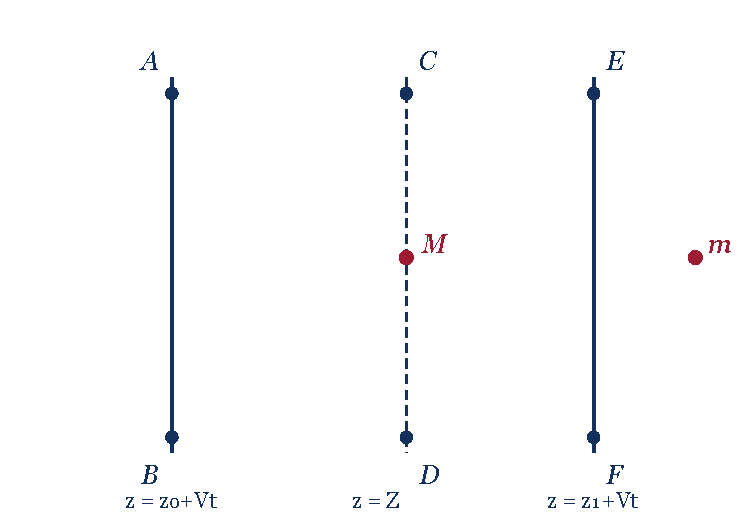
\includegraphics[width=0.7\textwidth]{figuras/pdf/cap02-fig1.pdf}
\caption{Los dos planos $z=z_0+\mathrm{V}t$ y $z=z_1+\mathrm{V}t$, con el
punto $\mathrm{M}$ interior y el punto $m$ exterior a la región
perturbada.}
\label{fig:vol2-cap2-1}
\end{figure}

\noindent\textbf{20.} Esta regla es todavía aplicable a una serie de
corrientes paralelas a $\mathrm{O}x$, como en el caso que nos ocupa.

Sea un punto $m$ exterior a los dos planos (figura~\ref{fig:vol2-cap2-1}):
consideremos una capa infinitamente delgada comprendida entre dos planos
$z$, y $z+dz$; podemos considerar la densidad $u$ de la corriente o de la
materia atrayente como constante en esta capa; y la atracción de esta
capa será la misma que la de un plano indefinido recubierto de materia
atrayente con una densidad superficial $\delta=u\,dz$. Se sabe que esta
atracción sobre un punto $m$ es constante e independiente de la distancia
de $m$ al plano y tiene por valor $2\pi\delta$.
\[
\delta=u\,dz=-\mathrm{V}\mathrm{F}'(z-\mathrm{V}t)\,dz.
\]

La atracción de toda la parte perturbada será:\footnote{El original
imprime $\mathrm{F}'(z-vt)$ en el integrando; es una errata evidente por
$\mathrm{F}'(z-\mathrm{V}t)$, pues $\mathrm{V}$ es la velocidad de la luz y
no hay ninguna otra velocidad en juego.~(N.~del T.)}
\[
\int_{z_0+\mathrm{V}t}^{z_1+\mathrm{V}t}-2\pi\mathrm{V}\mathrm{F}'(z-\mathrm{V}t)\,dz
=-2\pi\mathrm{V}\bigl[\mathrm{F}(z-\mathrm{V}t)\bigr]_{z_0+\mathrm{V}t}^{z_1+\mathrm{V}t}.
\]

Pero por hipótesis $\mathrm{F}(z_0)=\mathrm{F}(z_1)=0$: luego la atracción
buscada es nula.

No hay, pues, fuerza magnética fuera de los dos planos y, por
consiguiente, no hay inducción.

Sea ahora un punto interior $\mathrm{M}$ que tenga por ordenada
$\mathrm{Z}$. Tracemos el plano $z=\mathrm{Z}$, tendremos dos regiones por
distinguir: la primera, $ABCD$, a la izquierda de ese plano; la segunda,
$CDEF$, a la derecha. La atracción de la porción de la izquierda es igual
en valor absoluto a\footnote{El original imprime como límite superior de
esta integral una $z$ minúscula; es una errata evidente por la ordenada
$\mathrm{Z}$ del punto $\mathrm{M}$, como muestra el segundo miembro.~(N.~del
T.)}
\[
-2\pi\mathrm{V}\int_{z_0+\mathrm{V}t}^{\mathrm{Z}}\mathrm{F}'(z-\mathrm{V}t)\,dz
=-2\pi\mathrm{V}\mathrm{F}(\mathrm{Z}-\mathrm{V}t),
\]
puesto que $\mathrm{F}(z_0)=0$.

La atracción de la porción de la derecha tiene por valor absoluto
\[
-2\pi\mathrm{V}\int_{\mathrm{Z}}^{z_1+\mathrm{V}t}\mathrm{F}'(z-\mathrm{V}t)\,dz
=+2\pi\mathrm{V}\mathrm{F}(\mathrm{Z}-\mathrm{V}t),
\]
puesto que $\mathrm{F}(z_1)=0$.

Pero estas dos atracciones, estando dirigidas en sentidos contrarios, sus
valores absolutos deben restarse: lo que da para el valor de la atracción
resultante:
\[
-4\pi\mathrm{V}\mathrm{F}(\mathrm{Z}-\mathrm{V}t).
\]

La fuerza magnética entre nuestros dos planos no es, pues, nula.
